\documentclass[compress]{beamer}
%\usepackage[danish]{babel}
\usepackage[latin1]{inputenc}
%\usepackage{beamerarticle}
\usepackage{beamerthemesplit}
\usepackage{graphicx}
\usetheme{Darmstadt}
%\usetheme{PaloAlto}
%\usetheme{Berkeley}
%\usetheme{Frankfurt}
%\usetheme{Hannover}

%\usepackage{SHmathnot}
%\usepackage{natbib}
%\usepackage{amsmath,amsfonts}
\usepackage{bm}
\usepackage{ISMLS}


\def\lmer{\texttt{lmer()}}
%% bold letter UHH:
\def\betab{\bm \beta}
\def\phib{\bm \phi}
\def\phiAhat{\bm {\hat \Phi}_A}
\def\Lb{\bm L}
\def\ssb{\bm{\hat \sigma}}
\def\sigmab{\bm{\sigma}}
\def\Sigmab{\bm{\Sigma}}

\DeclareMathOperator{\var}{\mathbb{V}ar}
\DeclareMathOperator{\cov}{\mathbb{C}ov}
\DeclareMathOperator{\EE}{\mathbb{E}}


\makeatletter\def\Hy@xspace@end{}\makeatother

\setbeamerfont{block body}{size=\scriptsize}
\setbeamertemplate{footline}[page number]

%\makeatletter
%\AtBeginPart{\beamer@tocsectionnumber=0\relax\c@section=0}
%\makeatother

\title{
Kenward-Roger modification of the F-statistic for some linear mixed 
models fitted with lmer
}
% \author{Ulrich Halekoh and S�ren H�jsgaard}
% \institute{Department of Molecular Biology and Genetics \\ Aarhus University, Denmark}


\author[shortname]{Ulrich Halekoh \inst{1} \and S�ren H�jsgaard \inst{2}} 
\institute[shortinst]{
  \inst{1} Department of Molecular Biology and Genetics \\ Aarhus University, Denmark\\
  \emph{ulrich.halekoh@agrsci.dk}
  \and 
  \inst{2} Department of Mathematical Sciences \\ Aalborg University, Denmark\\  
  \emph{sorenh@math.aau.dk}} 
  


\newenvironment{sframe}
                {\begin{frame} [containsverbatim] }
                {\hfill  \end{frame}}

\newenvironment{sblock}
                 {\begin{block} {R-code} }
                 {\hfill  \end{block}}


\usepackage{Sweave}
\begin{document}

\frame{\titlepage}

\parskip4pt
\section*{Contents}
\begin{frame}
 \setcounter{framenumber}{1}
  \tableofcontents
\end{frame}







\section{Outline}
\label{sec:xxx}

\subsection{Motivation: Sugar beets - A split--plot experiment}
\label{sec:xxx}

\begin{sframe}
  \begin{itemize}
  \item   Dependence of  sugar percentage of sugar beets on
  harvest time and sowing time is investigated.

\item Five sowing times ($s$) and two harvesting times ($h$).


\item Experiment was laid out in three blocks ($b$).

  \end{itemize}

{\tiny
\begin{verbatim}
Experimental plan for sugar beets experiment

Sowing times:
  1: 4/4, 2: 12/4, 3: 21/4, 4: 29/4, 5: 18/5

Harvest times:
  1: 2/10, 2: 21/10

Plot allocation:
      |  Block 1           |  Block 2           |  Block 3           |
      +--------------------|--------------------|--------------------+
Plot  | h1  h1  h1  h1  h1 | h2  h2  h2  h2  h2 | h1  h1  h1  h1  h1 | Harvest time
 1-15 | s3  s4  s5  s2  s1 | s3  s2  s4  s5  s1 | s5  s2  s3  s4  s1 | Sowing time
      |--------------------|--------------------|--------------------|
Plot  | h2  h2  h2  h2  h2 | h1  h1  h1  h1  h1 | h2  h2  h2  h2  h2 | Harvest time
16-30 | s2  s1  s5  s4  s3 | s4  s1  s3  s2  s5 | s1  s4  s3  s2  s5 | Sowing time
      +--------------------|--------------------|--------------------+
\end{verbatim}
}

\end{sframe}

\begin{sframe}

% Let $h$ denote harvest time ($h=1,2$), $b$ denote block
% ($b=1,2,3$) and $s$ denote sowing time ($s=1,\dots,5$). Let $H=2$,
% $B=3$ and $S=5$.

  \begin{itemize}
  \item 
For simplicity we assume that there is no interaction between sowing
and harvesting times.


\item A typical model for such an experiment would be:
\begin{equation}
  \label{eq:beetsmodel1}
  y_{hbs} = \mu + \alpha_h + \beta_b + \gamma_s + U_{hb} + \epsilon_{hbs},
\end{equation}
where $U_{hb} \sim N(0,\omega^2)$ and $\epsilon_{hbs}\sim
N(0,\sigma^2)$.


\item Notice that $U_{hb}$ describes the random variation
between whole--plots (within blocks).

  \end{itemize}

\end{sframe}


\begin{sframe}

As the design is balanced we may make F--tests for each of the effects
as:
\begin{sblock}
\begin{Schunk}
\begin{Sinput}
> beets$bh <- with(beets, interaction(block, harvest))
> summary(aov(sugpct~block+sow+harvest+Error(bh), beets))
\end{Sinput}
\begin{Soutput}
Error: bh
          Df Sum Sq Mean Sq F value Pr(>F)
block      2 0.0327  0.0163    2.58   0.28
harvest    1 0.0963  0.0963   15.21   0.06
Residuals  2 0.0127  0.0063               

Error: Within
          Df Sum Sq Mean Sq F value  Pr(>F)
sow        4   1.01  0.2525     101 5.7e-13
Residuals 20   0.05  0.0025                
\end{Soutput}
\end{Schunk}
\end{sblock}

Notice: the F--statistics are $F_{1,2}$ for harvest time and $F_{4,20}$ for
sowing time.
\end{sframe}

\begin{sframe}

Using \code{lmer()} from \pkg{lme4} we can
fit the models and test for no effect of sowing and harvest time as follows:

\begin{sblock}

\begin{Schunk}
\begin{Sinput}
> beetLarge<-lmer(sugpct~block+sow+harvest+(1|block:harvest),
+             data=beets, REML=FALSE)
> beet_no.harv <- update(beetLarge, .~.-harvest)
> beet_no.sow  <- update(beetLarge, .~.-sow)
> as.data.frame(anova(beetLarge, beet_no.sow))
\end{Sinput}
\begin{Soutput}
            Df     AIC     BIC logLik deviance Chisq Chi Df Pr(>Chisq)
beet_no.sow  6  -2.795   5.612  7.398    -14.8    NA     NA         NA
beetLarge   10 -79.998 -65.986 49.999   -100.0  85.2      4  1.374e-17
\end{Soutput}
\begin{Sinput}
> as.data.frame(anova(beetLarge, beet_no.harv))
\end{Sinput}
\begin{Soutput}
             Df    AIC    BIC logLik deviance Chisq Chi Df Pr(>Chisq)
beet_no.harv  9 -69.08 -56.47  43.54   -87.08    NA     NA         NA
beetLarge    10 -80.00 -65.99  50.00  -100.00 12.91      1  0.0003261
\end{Soutput}
\end{Schunk}
\end{sblock}

The LRT based $p$--values are anti--conservative: the effect
of harvest appears stronger than it is.

\end{sframe}



\subsection{Motivation: A random regression problem}
\begin{sframe}
  \frametitle{Random coefficient model}
The change with age  of the distance between two cranial
distances was
observed for 16 boys and 11 girls
from age 8 until age 14.

\begin{figure}[ht]
 \centering
 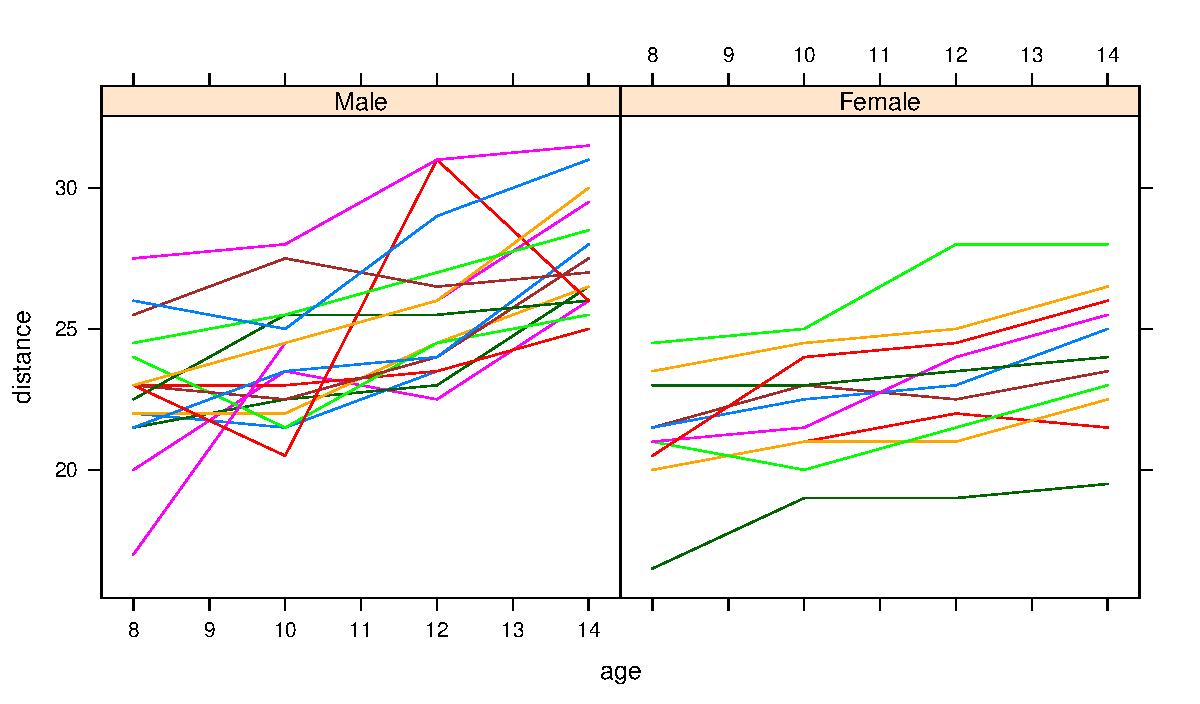
\includegraphics[width=0.9\textwidth]{fig/ortfig01}\\[-0.5cm]
%%\caption{Orthodont data}
 \label{fig:ortfig01}
\end{figure}
\end{sframe}

\begin{sframe}
  \frametitle{Random coefficient model}
  Plot suggests:
\[
dist_{[i]} = \alpha_{sex[i]}
+ \beta_{sex[i]} age_{[i]} + A_{Subj[i]} +
B_{Subj[i]} age_{[i]} + e_{[i]}
\]
with $(A,B) \sim N(0,\bm S)$.

ML-test of $\beta_{boy}=\beta_{girl}$:
\begin{sblock}
\begin{Schunk}
\begin{Sinput}
> ort1ML<- lmer(distance ~ age + Sex + age:Sex + (1 + age | Subject),
+                   REML = FALSE, data=Orthodont)
> ort2ML<- update(ort1ML, .~.-age:Sex)
> as.data.frame(anova(ort1ML, ort2ML))
\end{Sinput}
\begin{Soutput}
       Df   AIC   BIC logLik deviance Chisq Chi Df Pr(>Chisq)
ort2ML  7 446.8 465.6 -216.4    432.8    NA     NA         NA
ort1ML  8 443.8 465.3 -213.9    427.8 5.029      1    0.02492
\end{Soutput}
\end{Schunk}
\end{sblock}
\end{sframe}



\subsection{Our goal}
\label{sec:our-goal}

\begin{sframe}
\frametitle{Our goal...}
  Our goal is to extend the tests provided by \lmer.

  There are two issues here:

  \begin{itemize}
  \item  The choice of test statistic and

  \item  The reference distribution in which the test statistic is evaluated.

  \end{itemize}

\end{sframe}



\section{The Kenward--Roger modification of the $F$--statistic}

\begin{sframe}
\frametitle{Setting the scene}
For multivariate normal data
\[
Y_{n\times 1} \sim  N(\bm X_{n\times p} \bm \beta_{p\times 1}, \bm \Sigma)
\]
we consider the test of the hypothesis
\[
\Lb_{l \times p} \betab = \bm \beta_0
\]
where $\Lb$ is a regular matrix of estimable functions of $\bm \beta$.

The linear hypothesis
can be tested via the  Wald-type  statistic
\begin{gather*}
F= \frac{1}{l}(\hat \betab - \betab_0)^\top \Lb^\top   (\Lb^\top \bm \Phi(\ssb) \Lb)^{-1}
 \Lb (\hat \betab - \betab_0)
\end{gather*}
\begin{itemize}
\item
$\bm \Phi (\sigmab) = (\bm X^\top \bm \Sigma(\sigmab) \bm X)^{-1} \approx
\cov(\hat \betab)$, $\hat  \betab$ REML estimate of $\betab$ 
\item
$\ssb$: vector of REML estimates of the elements of $\Sigmab$
\end{itemize}
\end{sframe}

%%\subsection{An ``F''--statistic}
\begin{sframe}
  \frametitle{Kenward and Roger's modification}
Kenward and Roger (1997) modify the test statistic
\begin{itemize}
\item
$\bm \Phi$ is replaced by an improved small sample approximation $\bm \Phi_A$
\end{itemize}
Furthermore
\begin{itemize}
\item   
the statistic $F$ is scaled by a factor $\lambda$,
\item
denominator degrees of freedom $m$ are determined
\end{itemize}
such that the approximate expectation and variance are those of a $F_{l,m}$ distribution.
\end{sframe}


\begin{sframe}
\frametitle{Restriction on covariance}
\begin{itemize}

\item 
Consider only situations where 
\begin{gather*}
\Sigmab= \sum_i \sigma_i \bm G_i, \quad \bm G_i \, \text{known matrices}
\end{gather*}


\item Variance component and random coefficient models satisfy this
restriction.


\item $\bm \Phi_A(\ssb)$  depends now only on the first  partial derivatives of $\bm \Sigma^{-1}$:
\begin{displaymath}
\frac{\partial \bm \Sigmab^{-1}}{\partial \sigma_i} =
-
\bm \Sigma^{-1}
\frac{\partial \bm \Sigmab}{\partial \sigma_i}
\bm \Sigma^{-1}.  
\end{displaymath}



\item $\bm \Phi_A(\ssb)$  depends also on $\var(\ssb)$.


\item Kenward and Roger propose to estimate
  $\var(\ssb)$ via the  inverse expected information matrix.

\end{itemize}

\end{sframe}


\begin{sframe}
  \frametitle{Properties of the Kenward--Roger adjustment}
The  modification of the F-statistic by Kenward and Roger
\begin{itemize}
\item
yields the exact F-statistic for balanced mixed classification nested models
or balanced split plot models (Alnosaier, 2007).
\item
Simulation studies (e.g. Spilke, J. et al.(2003)) indicate that the Kenward-Roger approach perform  mostly better than alternatives  (like Satterthwaite  or containment method) for blocked experiments even with missing data. 
\end{itemize}
\end{sframe}



\begin{sframe}
  \frametitle{{{\bf R} package \tt lme4}}
The R package lme4 (Bates, D., Maechler, M,  Bolker, B., 2011)
provides efficient estimation of linear mixed models.

The package provides all necessary matrices and estimates
 to  implement the Kenward-Roger approach.


\begin{enumerate}
\item
The implementation uses a  straightforward transcription of the
description in the article of Kenward and Roger,  1997.
\item
Matrix operations use sparse matrices representation.
\item
Matrices are extracted from \verb+lmer+ objects via their slots (using \verb+@+).
\end{enumerate}
\end{sframe}




\begin{sframe}
  \frametitle{Kenward--Roger: split-plot (sugar-beets)}
The Kenward--Roger approach yields the same results
as the anova-test:
\begin{sblock}
\begin{Schunk}
\begin{Sinput}
> beetLarge <- update(beetLarge, REML=TRUE)
> beet_no.harv <- update(beet_no.harv, REML=TRUE)
\end{Sinput}
\end{Schunk}
\end{sblock}
Test for harvest effect:
\begin{sblock}
\begin{Schunk}
\begin{Sinput}
> KRmodcomp(beetLarge,beet_no.harv)
\end{Sinput}
\begin{Soutput}
F-test with Kenward-Roger approximation; computing time: 0.06 sec.
large : sugpct ~ block + sow + harvest + (1 | block:harvest)
small : sugpct ~ block + sow + (1 | block:harvest)
      stat  ndf  ddf F.scaling p.value
Ftest 15.2  1.0  2.0         1    0.06
\end{Soutput}
\end{Schunk}
\end{sblock}
\end{sframe}

\begin{sframe}
  \frametitle{Kenward--Roger:  random regression (cranial change)}
For the cranial distances  data the
Kenward and Roger modified F-test yields
\begin{sblock}
\begin{Schunk}
\begin{Sinput}
> ort1<- update(ort1ML, .~., REML = TRUE)
> ort2<- update(ort2ML, .~., REML = TRUE)
> KRmodcomp(ort1,ort2)
\end{Sinput}
\begin{Soutput}
F-test with Kenward-Roger approximation; computing time: 0.13 sec.
large : distance ~ age + Sex + (1 + age | Subject) + age:Sex
small : distance ~ age + Sex + (1 + age | Subject)
       stat   ndf   ddf F.scaling p.value
Ftest  5.12  1.00 25.52         1   0.032
\end{Soutput}
\end{Schunk}
\end{sblock}
The p-value form the ML-test was 0.0249.
\end{sframe}



\section{Parametric bootstrap}
\begin{sframe}
\frametitle{Using parametric bootstrap}

\begin{itemize}
\item 
The Kenward--Roger approach is no panacea.
\item
Additionally, we provide  
the parametric bootstrap p-value
  $P_{\hat\theta_0}(T \ge t_{obs})$ based on the log-LR statistic $T$.
\end{itemize}
  
We  draw $B$ parametric bootstrap samples
$t^1, \dots, t^B$ under the  estimated null model $\hat \theta_0$
and provide three choices to calculate the p-value.
 
\end{sframe}

\begin{sframe}
\begin{enumerate}
\item
directly via the proportion of sampled $t_i$ exceeding $t_{obs}$, 
\item
approximating the distribution of the scaled statistic $\frac{f}{\bar t}\cdot T$ by
a  $\chi^2_f$ distribution (Bartlett type correction)\\
($\bar t$ is the sample average  and $f$ the difference in the number of parameters
between the null and the alternative model)  
\item
approximating the bootstrap distribution by a $\Gamma(\alpha,\beta)$ distribution
which mean and variance match the moments of the bootstrap sample.
\end{enumerate}


\begin{sblock}
\begin{Schunk}
\begin{Sinput}
> PBmodcomp(beetLarge,beet_no.harv)
\end{Sinput}
\begin{Soutput}
Parametric bootstrap test; time: 20.00 sec; samples: 1000 extremes: 44;
large : sugpct ~ block + sow + harvest + (1 | block:harvest)
small : sugpct ~ block + sow + (1 | block:harvest)
       stat df p.value
LRT    11.8  1 0.00059
PBtest 11.8    0.04496
\end{Soutput}
\end{Schunk}
\end{sblock}

\end{sframe}



\begin{sframe}
Results from sugar beets:
\input{pvalbeets.txt}

Results for cranial distance data:
\input{pvalorto.txt}
\end{sframe}




\section{Small simulation study: A random regression problem}
\begin{sframe}
  \frametitle{Random coefficient model}
We consider the simulation from  a simple random coefficient model
(cf. Kenward  and Roger (1997, table 4)):
\begin{gather*}
y_{it}= \beta_0 + \beta_1 \cdot t_i  + A_{i} + B_i \cdot t_i + \epsilon_{it}
\end{gather*}
with $cov(A_i,B_{i})=
\left[
\begin{array}{rr}
 0.250 & -0.133\\
-0.133 &  0.250
\end{array}
\right] $
and $var(\epsilon_{it})=0.25$.

There are observed $i=1,\dots,24$ subjects divided in groups of 8.
For each group observations are
at the non overlapping times $t=0, 1, 2; t=3, 4, 5$ and $t=6, 7, 8$.
\end{sframe}




\begin{sframe}
  \frametitle{Results from random coefficient model}
\input{pvalrandcof2.txt}
\end{sframe}


\section{Final remarks}
\label{sec:final-remarks}

\begin{sframe}
  \frametitle{Summary}

  \begin{itemize}
  \item   The functions \verb'KRmodcomp()' and \verb'PBmodcomp()' 
    described here are available in the \verb+pbkrtest+ package.

    
  \item The Kenward--Roger approach requires fitting by REML; the parametric
  bootstrap approaches requires fitting by ML.


\item The required fitting scheme is set by the relevant functions, so the
  user needs not worry about this.


\item Parametric bootstrap is parallelized using the \verb'snow'
  package. 
  
  \end{itemize}
  

\end{sframe}





% \subsection{Speeding up: Sequential and parallel evaluations}

% \begin{sframe}

%   The above approaches are computationally intensive but there are
%   possibilities for speedups:

%   Instead of simulating a fixed number of values $t^1, \dots, t^M$ for
%   determining the reference distribution used for finding $p^{PB}$
%   we may instead introduce a stopping rule saying \emph{simulate until we
%   have found, say 20 values $t^j$ larger than $t_{obs}$.} If $J$
%   simulations are made then the reported $p$--value is $20/J$.

%   Estimating tail--probabilities will require more samples than
%   estimating the mean (and variance) of the reference
%   distribution. Therefore the Bartlett and gamma approaches will
%   require fewer simulations than needed for finding $p^{PB}$.

%   The simulation of the reference distribution can be parallelized
%   onto different processors.


% \end{sframe}


\begin{sframe}
  \frametitle{Literature}

\begin{itemize}
\item
Alnosaier, W. (2007) 
\textit{Kenward-Roger Approximate F Test for Fixed Effects in Mixed Linear Models}, Dissertation, Oregon State University  
\item
Bates, D., Maechler, M.  and Bolker, B. (2011)
\textit{lme4: Linear mixed-effects models using S4 classes},
R package version 0.999375-39.
\item
Kenward,  M. G. and Roger, J. H. (1997)
\textit{Small Sample Inference for Fixed Effects from Restricted Maximum Likelihood},
Biometrics, Vol. 53, pp. 983--997                    
\item
Spilke J., Piepho, H.-P. and Hu, X. Hu (2005)
\textit{A Simulation Study on Tests of Hypotheses
and Confidence Intervals for Fixed Effects in
Mixed Models for Blocked Experiments With
Missing Data}
Journal of Agricultural, Biological, and Environmental Statistics,
Vol. 10,p. 374-389
\end{itemize}
\end{sframe}


\end{document}

